\begin{frame}{Step 1: Research and Analysis}
	\begin{itemize}
		\item \textbf{Exploring GEM5 Internals:}
		      \begin{itemize}
			      \item Investigated the core components of GEM5 including CPU models, memory systems, and simulation flow.
			      \item Found limited developer documentation — referred to the official \href{https://doxygen.gem5.org/develop/index.html}{Doxygen documentation \faLink}.
			      \item Studied through 3,358 source files comprising 965,657 lines of code.
		      \end{itemize}

		\item \textbf{Studying AVR Architecture:}
		      \begin{itemize}
			      \item Reviewed instruction set, register architecture, and interrupt handling for AVR microcontrollers.
		      \end{itemize}

		\item \textbf{Feasibility Analysis:}
		      \begin{itemize}
			      \item Evaluated how a lightweight 16-bit AVR ISA could be integrated into GEM5’s CPU model framework.
			      \item Focused on maintaining modularity and clean abstraction layers.
		      \end{itemize}

		\item \textbf{Initial Outcomes:}
		      \begin{itemize}
			      \item Conducted a simulation-based evaluation titled \href{https://drive.google.com/file/d/13ZroHuWGLApYXLkeWA3SBIlMh6KzfCqq/view?usp=sharing}{\texttt{Comparative Study on Execution Speed \& CMR of Various ISAs \faLink.}}
		      \end{itemize}
	\end{itemize}
\end{frame}

\begin{frame}{Exploring Gem5 Internals}
	\begin{itemize}
		\item We studied the effect of architecture and cache configuration on execution speed and CMR.
		\item We studied on Matrix Multiplication algorithm.
		\item Following parameters were varied:
		      \begin{table}[ht]
			      \centering
			      \footnotesize
			      \renewcommand{\arraystretch}{1.1}
			      \begin{tabularx}{14cm}{|>{\centering\arraybackslash}m{3cm}|>{\centering\arraybackslash}m{4cm}|>{\centering\arraybackslash}m{5.7cm}|}
				      \hline
				      \textbf{Parameters} & \textbf{Values}        & \textbf{Description}                                     \\
				      \hline
				      Architecture        & ARM, RISC-V, x86       & Instruction Set Architecture type used in the simulation \\
				      \hline
				      Cache Availability  & Yes, No                & Whether cache memory is available in the simulation      \\
				      \hline
				      L1D Size            & 32, 64, 128 kB         & Size of Level 1 data cache                               \\
				      \hline
				      L1I Size            & 32, 64, 128 kB         & Size of Level 1 instruction cache                        \\
				      \hline
				      L2 Size             & 128, 256, 512, 1024 kB & Size of Level 2 cache                                    \\
				      \hline
				      Matrix Dimension    & 5, 10, 20, 40, 80      & Dimension of the square matrix for multiplication        \\
				      \hline
				      max\_val            & $10^6$                 & Maximum absolute value of the elements in the matrix     \\
				      \hline
			      \end{tabularx}
			      \vspace{0.2cm}
			      \caption{Parameters of Simulation}
			      \label{tab:sim_params}
		      \end{table}
	\end{itemize}
\end{frame}

\begin{frame}{Exploring Gem5 Internals}
	\begin{itemize}
		\item In the meantime we monitored following parameters:
		      \begin{table}
			      \centering
			      \footnotesize
			      \renewcommand{\arraystretch}{1.2}
			      \begin{tabularx}{14cm}{|>{\ttfamily}l|X|}
				      \hline
				      \textbf{Parameter}              & \textbf{Description}                                 \\
				      \hline
				      \multicolumn{2}{|l|}{\textbf{Simulation Metrics}}                                      \\
				      \hline
				      simSeconds                      & Simulation time in seconds                           \\
				      \hline
				      simTicks                        & Simulated ticks                                      \\
				      \hline
				      simInsts                        & Number of instructions simulated                     \\
				      \hline
				      simOps                          & Number of operations simulated (including micro-ops) \\
				      \hline
				      core.cpi                        & Cycles per instruction                               \\
				      \hline
				      core.ipc                        & Instructions per cycle                               \\
				      \hline
				      \multicolumn{2}{|l|}{\textbf{L1 Data Cache}}                                           \\
				      \hline
				      l1d-cache-0.demandHits::total   & Total hits to L1 data cache                          \\
				      \hline
				      l1d-cache-0.demandMisses::total & Total misses to L1 data cache                        \\
				      \hline
				      \multicolumn{2}{|l|}{\textbf{L1 Instruction Cache}}                                    \\
				      \hline
				      l1i-cache-0.demandHits::total   & Total hits to L1 instruction cache                   \\
				      \hline
				      l1i-cache-0.demandMisses::total & Total misses to L1 instruction cache                 \\
				      \hline
			      \end{tabularx}
			      \vspace{0.1cm}
			      \caption{Target parameters to be monitored}
			      \label{tab:monitored_params1}
		      \end{table}
	\end{itemize}
\end{frame}




\begin{frame}{Exploring Gem5 Internals}
	\begin{table}
		\centering
		\footnotesize
		\renewcommand{\arraystretch}{1.2}
		\begin{tabularx}{14cm}{|>{\ttfamily}l|X|}
			\hline
			\textbf{Parameter}             & \textbf{Description}     \\
			\hline
			\multicolumn{2}{|l|}{\textbf{L2 Cache}}                   \\
			\hline
			l2-cache-0.demandHits::total   & Total hits to L2 cache   \\
			\hline
			l2-cache-0.demandMisses::total & Total misses to L2 cache \\
			\hline
		\end{tabularx}
		\vspace{0.1cm}
		\caption{Target parameters to be monitored}
		\label{tab:monitored_params2}
	\end{table}
	\begin{itemize}
		\item We simulated 555 different configurations and gathered the results.
		\item Each simulation produces a \texttt{m5out} directory containing the system configuration diagram and \texttt{stats.txt} containing the results.
	\end{itemize}
\end{frame}


\begin{frame}{Exploring Gem5 Internals}
	\begin{figure}[h]
		\centering
		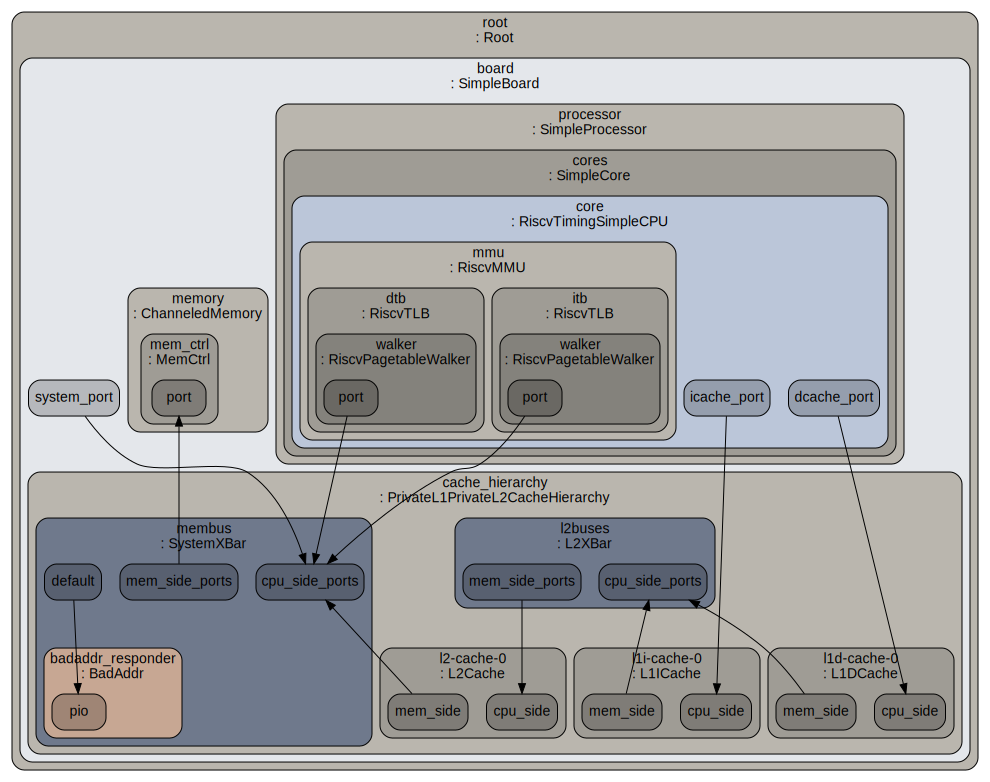
\includegraphics[width=7.5cm]{images/config.dot.png}
		\caption{Sample System Configuration Diagram}
		\label{fig:system_config}
	\end{figure}
\end{frame}

\begin{frame}[fragile]{Exploring Gem5 Internals}

	\begin{lstlisting}[language=C++, caption={Sample \texttt{stats.txt}}]
    ---------- Begin Simulation Statistics ----------
    simSeconds                                   0.000282                       # Number of seconds simulated (Second)
    simTicks                                    281722000                       # Number of ticks simulated (Tick)
    finalTick                                   281722000                       # Number of ticks from beginning of simulation (restored from checkpoints and never reset) (Tick)
    simFreq                                  1000000000000                       # The number of ticks per simulated second ((Tick/Second))
                                ...
  \end{lstlisting}
	\begin{itemize}
		\item The data is later gathered in a single file for comparison.
	\end{itemize}
\end{frame}

\begin{frame}
	\frametitle{Execution Performance Comparison}
	\begin{itemize}
		\item ARM ISA is most efficient with $\approx 16\%$ fewer instructions than RISC-V
		\item x86 requires $\approx 11\%$ more instructions than ARM
	\end{itemize}

	\begin{figure}[h]
		\centering
		\includegraphics[width=0.4\linewidth]{images/inst_count.png}
		\includegraphics[width=0.4\linewidth]{images/exec.png}
		\caption{Left: Simulated instruction count \quad Right: Execution time}
	\end{figure}
\end{frame}

\begin{frame}
	\begin{itemize}
		\item Execution time proportional to instruction count (same clock cycle time)
		\item x86 deviation due to higher opcode count (RISC ISAs are denser)
	\end{itemize}
\end{frame}

\begin{frame}[fragile]
	\frametitle{Cache Performance Metrics}
	\begin{columns}
		\begin{column}{0.5\textwidth}
			Cache miss rate calculation:
			\begin{equation*}
				\mathrm{miss\_rate} = \frac{\mathrm{misses}}{\mathrm{misses} + \mathrm{hits}}
			\end{equation*}

			\begin{table}[h]
				\centering
				\caption{Cache Performance Classification}
				\begin{tabular}{ll}
					\toprule
					Hit Rate Range & Interpretation     \\
					\midrule
					$>90\%$        & Excellent locality \\
					$60-90\%$      & Partial fit        \\
					$<60\%$        & Poor utilization   \\
					\bottomrule
				\end{tabular}
			\end{table}
		\end{column}

		\begin{column}{0.4\textwidth}
			\begin{figure}[h]
				\includegraphics[width=\linewidth]{images/op_count.png}
				\caption{Operation Count per ISA}
			\end{figure}
		\end{column}
	\end{columns}

	\begin{itemize}
		\item RISC family shows best cache performance
		\item L1I has the lowest miss rate (frequently accessed instructions)
	\end{itemize}
\end{frame}

\begin{frame}
	\frametitle{Cache Hierarchy Performance}
	\begin{columns}
		\begin{column}{0.5\linewidth}
			\begin{itemize}
				\item L1D also shows low miss rates (good data locality)
				\item L2 has higher miss rates (stores less frequent data)
			\end{itemize}
		\end{column}
		\begin{column}{0.4\linewidth}
			\begin{figure}[h]
				\centering
				\includegraphics[width=\linewidth]{images/l1i.png}
				\caption{L1 Instruction Cache Performance}
			\end{figure}
		\end{column}
	\end{columns}
\end{frame}

\begin{frame}
	\frametitle{Working Set Analysis}
	\begin{columns}
		\begin{column}{0.4\textwidth}
			\begin{figure}[h]
				\includegraphics[width=\linewidth]{images/l1d.png}
				\caption{L1 Data Cache Performance}
			\end{figure}
		\end{column}

		\begin{column}{0.4\textwidth}
			\begin{figure}[h]
				\includegraphics[width=\linewidth]{images/l2.png}
				\caption{L2 Cache Performance}
			\end{figure}
		\end{column}
	\end{columns}
\end{frame}

\begin{frame}
	\frametitle{Working Set Analysis}
	\begin{columns}
		\begin{column}{0.45\linewidth}
			\begin{figure}[h]
				\centering
				\includegraphics[width=0.5\linewidth]{images/dim_cache.png}
				\caption{Cache performance vs matrix size}
			\end{figure}
		\end{column}
		\begin{column}{0.4\linewidth}
			\begin{itemize}
				\item Hit rate increases with matrix size (more data reuse)
				\item Demonstrates importance of working set fitting in cache
			\end{itemize}
		\end{column}
	\end{columns}
\end{frame}
\begin{frame}[fragile]
  \frametitle{Insights into gem5 Internals}
  
  \begin{block}{Key Learnings About gem5 Architecture}
  \begin{itemize}
      \item \textbf{Simulation Methodology}:
      \begin{itemize}
          \item Verified gem5's cycle-accurate simulation approach
          \item Observed direct correlation between instruction count and execution time
          \item Validated statistical sampling methods
      \end{itemize}
      
      \item \textbf{Cache Hierarchy Modeling}:
      \begin{itemize}
          \item Demonstrated L1/L2 miss penalty differences
          \item Verified replacement policy implementations
          \item Analyzed coherence protocol overheads
      \end{itemize}
  \end{itemize}
  \end{block}
  
  \begin{exampleblock}{Validated gem5 Components}
  \begin{itemize}
      \item CPU models (TimingSimpleCPU/O3CPU)
      \item Memory access scheduling logic
      \item Cache prefetching algorithms
  \end{itemize}
  \end{exampleblock}
  \end{frame}
  
  \begin{frame}[fragile]
  \frametitle{Insights into gem5 Internals}
  
  \begin{columns}
  \begin{column}{0.45\textwidth}
  \begin{alertblock}{Architectural Insights}
  \begin{itemize}
      \item \textbf{ISA Differences}:
      \begin{itemize}
          \item Pipeline modeling accuracy verification
          \item Instruction decoding overheads
          \item Micro-op fusion effects
      \end{itemize}
      
      \item \textbf{Memory System}:
      \begin{itemize}
          \item Address translation costs
          \item DRAM controller behavior
          \item QoS implementation
      \end{itemize}
  \end{itemize}
  \end{alertblock}
  \end{column}
  
  \begin{column}{0.45\textwidth}
  \begin{block}{Practical Applications}
  \begin{itemize}
      \item Identified memory subsystem bottlenecks
      \item Developed ISA-specific optimization guidelines
      \item Created validation test suite
      \item Improved configuration templates
  \end{itemize}
  \end{block}
  \end{column}
  \end{columns}
  \end{frame}

\begin{frame}{Step 2: ISA Integration}
	\centering
	\includegraphics[width=0.55\textwidth]{images/impl.png}\\
	\textbf{Figure 3: }Dependence of gem5 components on ISA
\end{frame}

\begin{frame}{Step 2: ISA Integration}
	\begin{itemize}
		\item For the project we need to implement:
		      \begin{itemize}
			      \item ISA Description
			      \item Decoder
			      \item Fault Interrupts
			      \item Predecoder
			      \item Python Bindings to CPU \& I/O models.
			      \item GUI for the simulator
		      \end{itemize}
		\item For the begging a set of basic instructions are being implemented:
		      \begin{itemize}
			      \item \textbf{Arithmetic Instructions:} ADD, SUB
		      \end{itemize}
		\item Current implementation includes:
		      \begin{itemize}
			      \item ISA Description with two above-mentioned instructions
			      \item \texttt{AVRFault} for fault handling
			      \item \textbf{Registers:} 32 general-purpose registers (R0-R31), SREG (Status Register)
			      \item \textbf{Program Counter (PC):} 16-bit PC for instruction addressing
			      \item \textbf{Instruction Fetch and Decode:} Basic fetch-decode-execute cycle
		      \end{itemize}
	\end{itemize}
\end{frame}

\begin{frame}[fragile]{Step 2: ISA Integration}
	\begin{figure}
		\centering
		\includegraphics[width=0.8\textwidth]{images/flow.png}\\
		\textbf{Figure 4:} ISA description flow
	\end{figure}
\end{frame}

\begin{frame}[fragile]{Step 2: ISA Integration}
	Traversing the pipeline with `\texttt{add}' instruction:
	\begin{itemize}
		\item Bitfield definition for the instructions to be later used in the decoder:
		      \begin{lstlisting}[language=C++]
        def bitfield OPCODE    <15:10>;
        def bitfield REG_D     <8:4>;
        def bitfield REG_R     <3:0>;
        def bitfield IMM8      <7:0>;
      \end{lstlisting}
	\end{itemize}
\end{frame}

\begin{frame}[fragile]{Step 2: ISA Integration}
	\begin{itemize}
		\item Format declaration for \texttt{add} instruction. The declaration defines the output blocks for the code to be generated:
		      \begin{lstlisting}[language=C++]
      def format Add(code, *opt_args) {{
        iop = InstObjParams(name, Name, 'AddOp',
                          {'code': code,
                            'predicate_test': predicateTest,
                            'op_class': 'gem5::enums::IntAlu'
                          },
                          opt_args)
        header_output = AddDeclare.subst(iop)
        decoder_output = AddConstructor.subst(iop)
        decode_block = AddDecode.subst(iop)
        exec_output = AddExecute.subst(iop)
        disasm_output = AddDisassembly.subst(iop)
    }};
    \end{lstlisting}
	\end{itemize}
\end{frame}

\begin{frame}[fragile]{Step 2: ISA Integration}
	\begin{itemize}
		\item Add class declaration including the constructor, execute method, disassembly method and PC advancement method:
		      \begin{lstlisting}[language=C++]
      def template AddDeclare {{
        class %(class_name)s : public gem5::AVRISAInst::AVRStaticInst
        {
          public:
            %(class_name)s(gem5::AVRISAInst::MachInst machInst);
            Fault execute(ExecContext *, trace::InstRecord *) const override;
            std::string generateDisassembly(Addr pc,
                const loader::SymbolTable *symtab) const override;
            void advancePC(PCStateBase &pc_state) const;
        };
      }};
    \end{lstlisting}
	\end{itemize}
\end{frame}

\begin{frame}[fragile]{Step 2: ISA Integration}
	\begin{itemize}
		\item Generated C++ code for the Add class from the DSL code above:
		      \begin{lstlisting}[language=C++]
      #undef OPCODE
      #define OPCODE	bits(machInst, 15, 10)
      #undef REG_D
      #define REG_D	bits(machInst,  8,  4)
      #undef REG_R
      #define REG_R	bits(machInst,  3,  0)
      #undef IMM8
      #define IMM8	bits(machInst,  7,  0)
      class Add : public gem5::AVRISAInst::AVRStaticInst
      {
        public:
          Add(gem5::AVRISAInst::MachInst machInst);
          Fault execute(ExecContext *, trace::InstRecord *) const override;
          std::string generateDisassembly(Addr pc,
              const loader::SymbolTable *symtab) const override;
          void advancePC(PCStateBase &pc_state) const;
      };
    \end{lstlisting}
	\end{itemize}
\end{frame}


\begin{frame}{Step 2: ISA Integration}
	\begin{itemize}
		\item Getting integration success with these two instructions opened door for further extending the instruction set.
		\item The groundwork for extension is laid out with the fault handling, PC management and register modeling.
	\end{itemize}
\end{frame}